\begin{figure}[h]
    \centering
    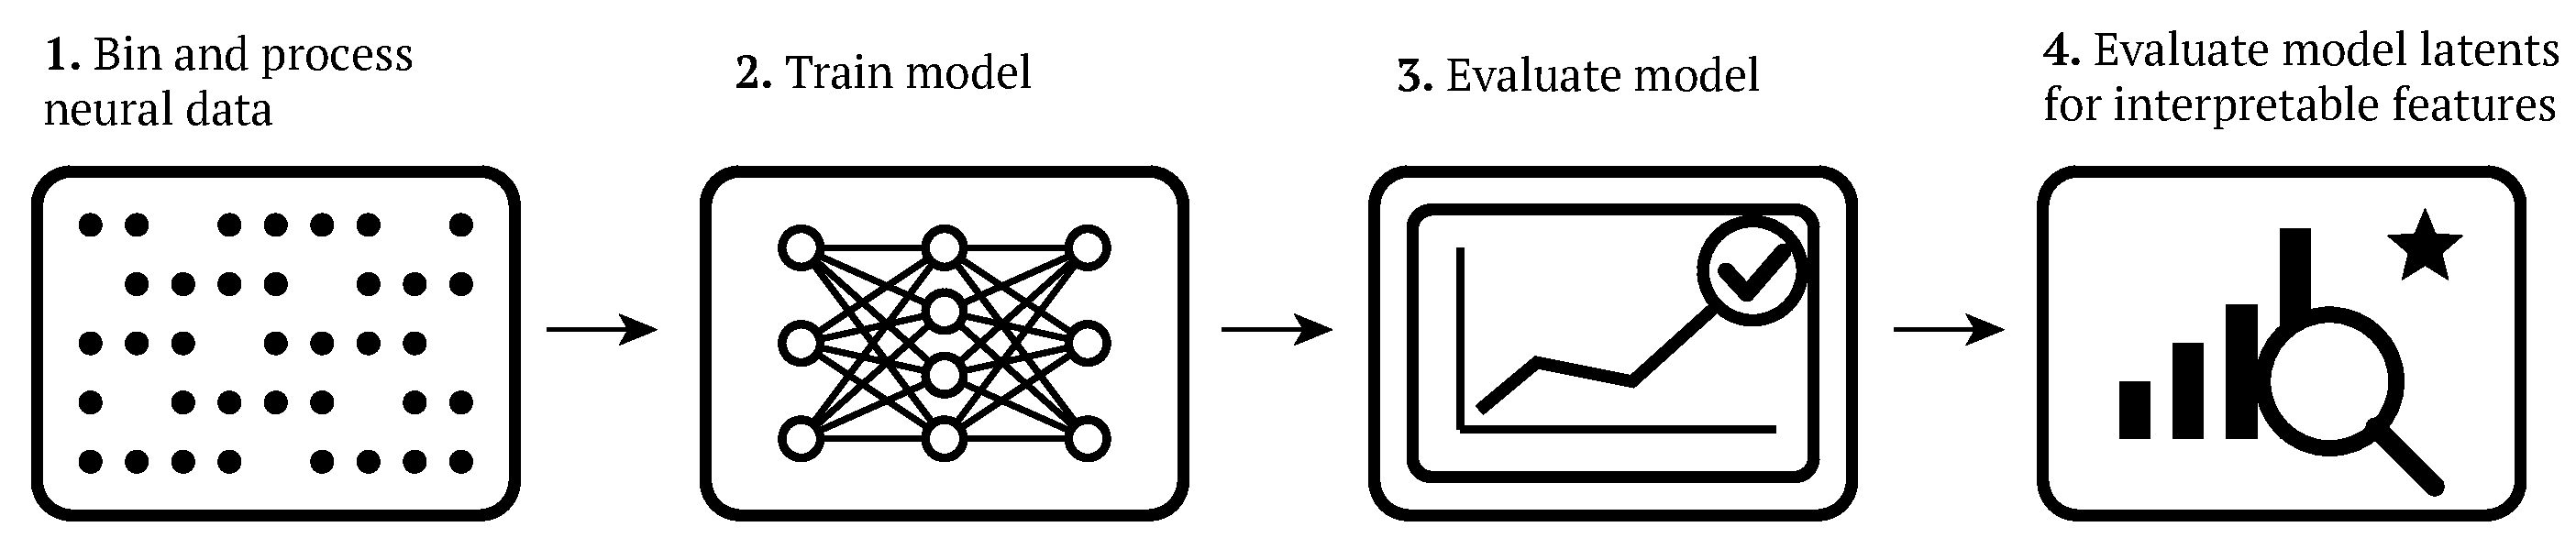
\includegraphics[width=\linewidth]{figures/mini_pipeline.pdf}
    \caption{
        \textbf{The MINI pipeline.} \\
        \small The MINI pipeline has 4 stages: 1) Spatiotemporal binning and processing of neural data; 2) Training a model; 3) Evaluating the model; 4) Evaluating the model's latents for feature interpretability. Steps 1-3 can be either semi- or fully-automated.
        \vspace{-1em}
    }
    \label{figure:mini_pipeline}
\end{figure}

\section{Methods: The MINI pipeline}

The MINI pipeline transforms high-dimensional neural data into a set of interpretable latents in four stages (\autoref{figure:mini_pipeline}), the first three of which can be fully automated.

\subsection{Data preprocessing}

The pipeline's first stage prepares neural data for model training. MINI includes utilities to process outputs from common spikesorters (e.g. Kilosort~\cite{pachitariu_2016_kilosort}) by aggregating, binning, and normalizing spike times into a 2D matrix of time by space, in which each bin contains neural activity from a neural unit for a specific time period. Normalization operations include min-max and z-scoring, applied across either the spatial or temporal dimension. This processing is readily adaptable to other forms of acquired neural data, such as ROIs from calcium imaging data processed by tools like Suite2p~\cite{pachitariu_2017_suite2p}. Alternatively, users may pass their own preprocessed neural data directly to the model training stage.

\begin{figure}[tbph]
    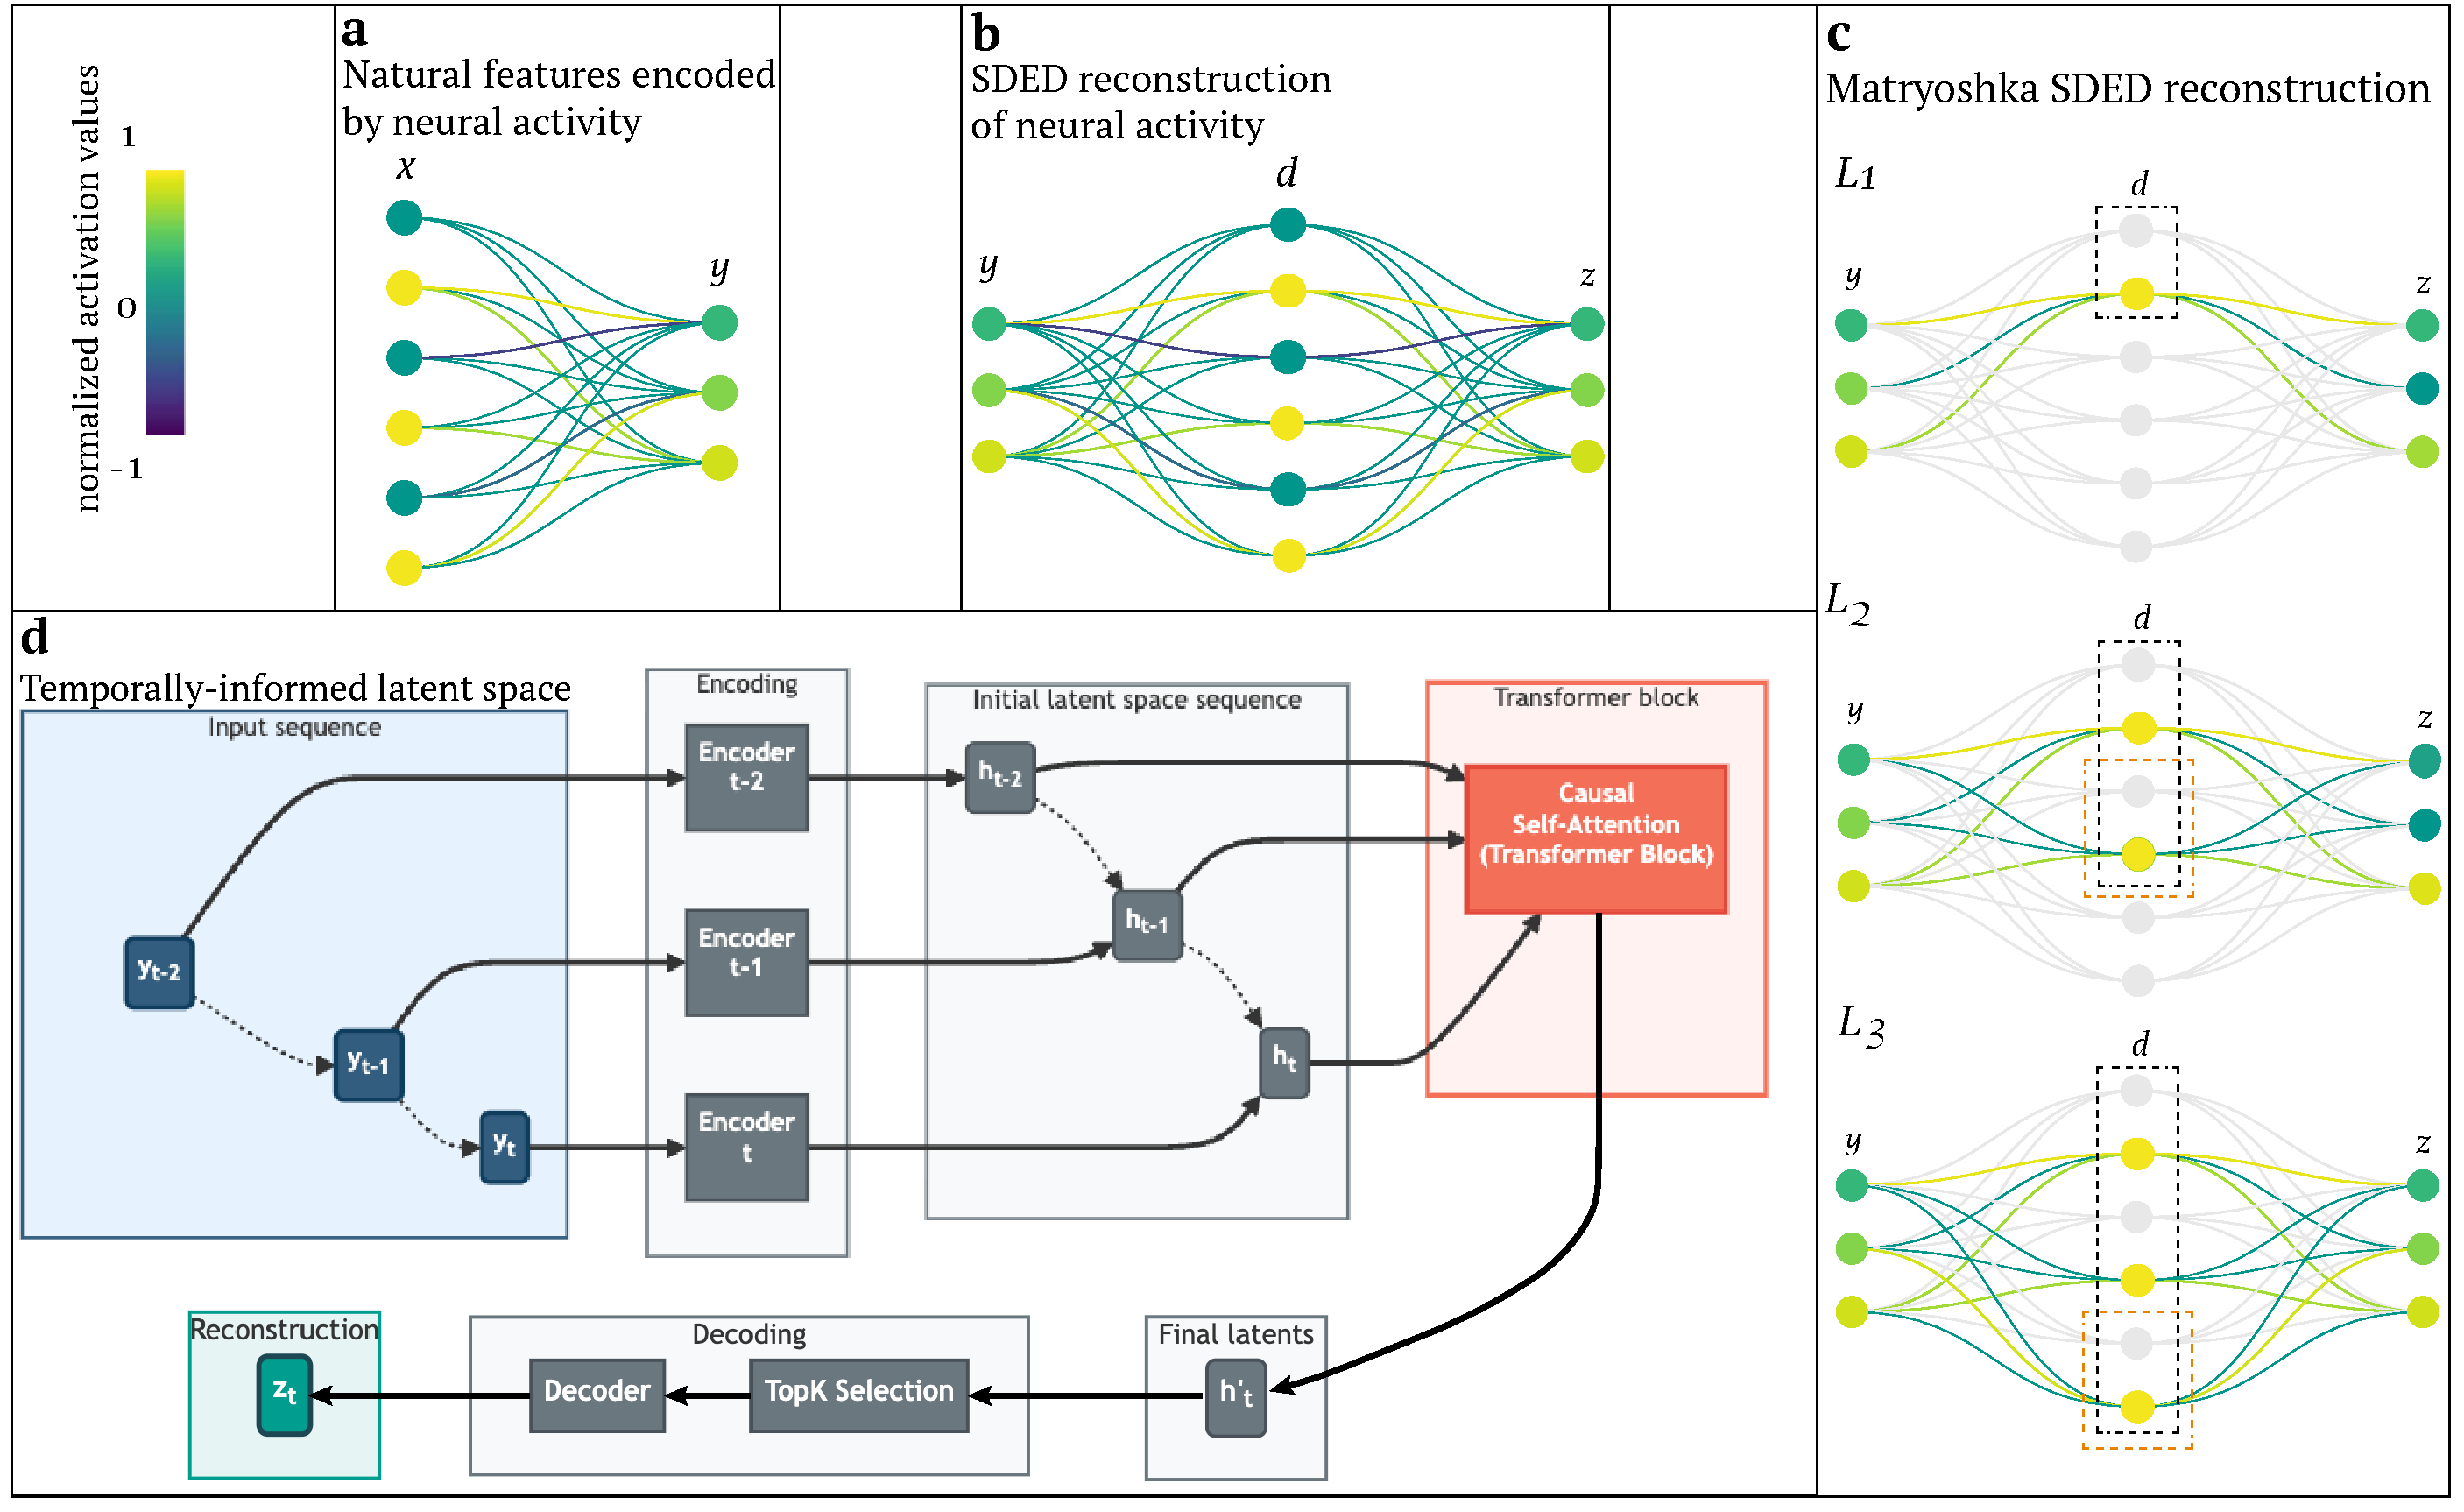
\includegraphics[width=\linewidth]{figures/sded_arch.pdf}
    \caption{
        \textbf{Model architecture considerations} \\
        \small
        (\textbf{a}) Natural, "real-world" features $x$ are encoded by neural activity $y$. In this example, three active features are simultaneously represented by the joint activity of three neurons. (\textbf{b}) A SDED reconstructs neural activity $z$ based on $y$ via sparse dictionary elements $d$. When training is successful, $d$ corresponds to $x$: sparse dictionary elements (i.e. model neurons) represent natural features. If $z$ tries to recreate $y$ exactly ($\hat{y}$), the model is an autoencoder; in other scenarios (e.g. $z$ is separate but dependent on or related to $y$) it is a transcoder or crosscoder. (\textbf{c}) A Matryoshka SDED segments the latent space into multiple nested levels, each of which attempts to do a full reconstruction of the target neural activity. The black boxes indicate the latents involved in a single level, while the light-red boxes indicate the additional latents used at lower-levels. In this example, $k$=1 for top-$k$ selection of latents to recruit for reconstruction at each level (the yellow neuron within each light-red box). Latents in the highest-level ($L_1$) will often correspond to high-level features (e.g. a round object), while latents exclusive to the lowest-level ($L_3$) will often correspond to low-level features (e.g. a basketball). (\textbf{d}) Incorporation of a transformer block with sequence input allows imbuing the latent space with temporal information corresponding to the evolution of the sequence, which can lead to improved reconstruction and interpretability. Each sample in the input sequence is transformed by the same encoding dictionary matrix in parallel to yield a latent space sequence. Causal self-attention is then performed on this sequence of latents via a single, small multi-head transformer block, yielding a final latent space. The latents are sparsified via top-k and transformed by the decoding dictionary matrix to yield the neural data reconstruction, as in the single, non-sequential input case.
        \vspace{-1em}
    }
    \label{figure:sded_arch}
\end{figure}

\subsection{Model training}

In stage 2, a SDED model is trained to reconstruct the processed neural data from latent, sparsely active dictionary elements -- the model's hidden layer neurons\footnote{In a SDED model: model neuron = dictionary element = latent}. The end goal is for these latents to represent disentangled, interpretable representations\footnote{In our vernacular: interpretable latent $\approx$ feature $\approx$ representation} encoded by the neural activity (\autoref{figure:sded_arch}a,b). Sparsity encourages the model to discover a monosemantic dictionary, in which each latent corresponds to a single feature. For instance, a latent from a model trained on visual cortex activity may correspond to a particular property of a visual stimulus, while a latent from a model trained on motor cortex activity may correspond to a specific aspect of movement.

The model can be configured as an autoencoder~\cite{cunningham_2023_saes} to reconstruct its own input (e.g. V1 activity based on V1 activity), or as a transcoder~\cite{ dunefsky_2024_transcoders} to reconstruct a dependent or related target of its input (e.g. V2 activity based on V1 activity, or V1 activity on day 2 based on V1 activity on day 1). These configurations allow for examining the intrinsic representational structure of a neural population and how representations may be transformed across brain regions and differ over time or between subjects. In each case, the model is trained to minimize the difference between the reconstructed and target neural data. The full training procedure is summarized in \nameref{algorithm:sded_model_training}. Here we discuss three key components: the batch top-$k$ sparsity, Matryoshka architecture, and integration over latent space history via self-attention.

A batch top-$k$ operator preserves only the $k \cdot B$ latents with the highest activation magnitudes across a batch of size $B$~\cite{bussmann_2024_batchtopk}. In contrast to indirect approaches that control latent sparsity (e.g. an L1 penalty), batch top-$k$ directly controls sparsity while flexibly permitting the number of active latents to vary per sample in the batch, aligning with the variable complexity of neural states. A novel variant of the Matryoshka SDED architecture~\cite{bussmann_2025_msae} segments the latent space into nested hierarchical levels, where each level attempts a full reconstruction of the target neural activity (\autoref{figure:sded_arch}c). This allows for multi-scale feature representation at single timepoints, and mitigates "feature absorption," a common issue where general features subsume specific ones~\cite{chanin_2024_feature_absorption}. For example, a model can learn that a "drifting grating" is a subset of the more general "grating" visual stimulus class without sacrificing the representation of either (\nameref{subsubsection:allen_dataset_results}). Lastly, if input data is provided as a sequence of timebins rather than a single timebin, an optional transformer block can integrate information over the latent space history via self-attention (\autoref{figure:sded_arch}d), enabling the model to learn features corresponding to evolving temporal dynamics, rather than just instantaneous neural patterns. 

The combination of these architectural options creates a flexible but large search space for model design. Searching this space effectively is crucial, as we empirically find that these components can significantly improve both reconstruction accuracy and feature interpretability (\nameref{subsubsection:model_architecture_details}). To streamline this search with minimal manual specification, MINI supports fully automated training via hyperparameter sweep configurations that support local or distributed training across one or multiple CPUs or GPUs (\nameref{subsubsection:hyperparameter_sweeps}).

\subsection{Model evaluation}

Folowing training, model quality is evaluated using a suite of quantitative metrics. MINI adapts the domain-general core metrics from the established mechanistic interpretability benchmark SAEBench~\cite{karvonen_2025_saebench}, and introduces others tailored for neural data. This stage serves as a critical checkpoint: while these metrics do not directly assess latent interpretability, they allow a researcher to determine if the model has learned a sparse, accurate, robust representation of the neural data. A model that performs well across these metrics is a strong candidate for the subsequent, final pipeline stage of evaluating individual latents.

Model evaluation centers on the trade-off between reconstruction fidelity and latent dictionary sparsity. High reconstruction fidelity is trivial to achieve with a large and dense code but undermines the goal of finding disentangled, interpretable latents. MINI therefore first reviews dictionary quality via latent sparsity metrics (\autoref{figure:model_eval} top). The mean L0 norm measures the average number of active latents per sample, set indirectly by the batch top-$k$ parameter, while the latent activity density visualizes the firing distribution across all latents. Together these metrics reveal whether the model has learned an efficient code that uses many latents intermittently while avoiding common pitfalls such as "representational collapse" into too many constantly active latents and/or widespread "feature death", in which a large portion of the dictionary never activates. These sparsity metrics are complemented by a couple of reconstruction fidelity metrics: variance explained (R\textsuperscript{2}) and cosine similarity of reconstruction-to-target neural activity across both spatial and temporal dimensions (\autoref{figure:model_eval} bottom). High scores in these metrics confirm that the sparse code is a sufficient representation that has captured salient information present in the target neural data.

For a deeper diagnosis, several optional metrics are available (\autoref{figure:model_eval_extra}). To check whether explanatory power is well-distributed, a variance attribution analysis quantifies the overall reconstruction variance explained by each individual latent. Additionally, to check if temporal information present in the target neural data is captured by the latents, a spectral frequency analysis compares the reconstruction's frequency content to that of the target neural data within a specified duration. 

Overall, these metrics provide a high-level overview of model quality, and to facilitate bespoke evaluation, the model's raw parameter, gradient, and activation data during training and evaluation are accessible.

\subsection{Latents evaluation}

Lastly in stage 4, the latents produced by the model are evaluated for interpretability. This can include visualizing their activation patterns over time and experimental conditions, as well as assessing their decoding performance. We detail typical approaches for exploring latents in \nameref{section:results}.
